\documentclass[9pt,t]{beamer}
% note that full page width is 12.8 cm and height is 9.6 cm

\mode<presentation>
{
  \usepackage[headline,footline]{beamerthemelectures}

}

% load packages
\usepackage[english]{babel}
\usepackage{graphicx}
\usepackage{multimedia}
%\usepackage[T1]{fontenc}
\usepackage{lmodern}
\usepackage{amsmath,amssymb}
\usepackage{pgf,booktabs,verbatim}
\usepackage{pgfarrows,pgfnodes}
\usepackage[absolute,overlay]{textpos}
\setlength{\TPHorizModule}{\paperwidth}
\setlength{\TPVertModule}{\paperheight}
\usepackage{tikz}

\setbeamertemplate{frametitle}{
\begin{centering}
\insertframetitle
\par
\end{centering}
} 

% create command to add nice looking citation
\newcommand{\reference}[1]{\flushright \vspace{-0.3cm} {\tiny #1}} 


\title{Solutions to Modeling Exercise \#5\\ Ice sheets}

\begin{document}

\section{}

%%%
\frame{
    \frametitle{\vspace{1cm}\huge Ice sheets} 
}

\frame{
\frametitle{1. Steady state/response time}
\begin{figure}
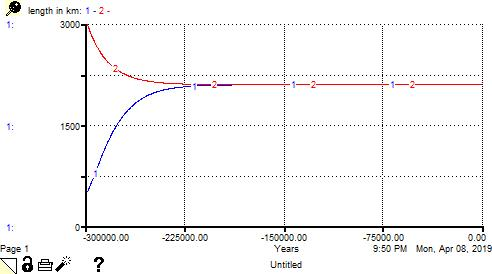
\includegraphics[width=0.8\textwidth]{./p1ab.jpg}
\end{figure}
\begin{itemize}
\item Evolves to a steady-state length of 2100 km.
\item Response time is on the order of 50 ka.
\end{itemize}
}

\frame{
\frametitle{2. Crossing threshold to rapid melting}
\begin{figure}
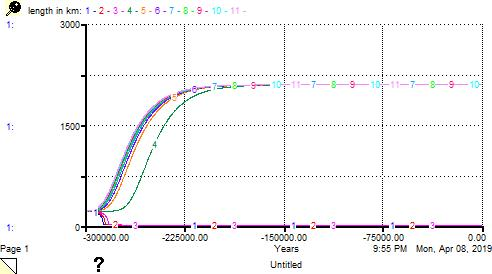
\includegraphics[width=0.8\textwidth]{./p2.jpg}
\end{figure}
\begin{itemize}
\item Threshold behavior at about 203 km.
\item Positive feedbacks dominate at lengths less than 203 km.
\end{itemize}
}

\frame{
\frametitle{3. Changing the grounding line/climate}
\begin{figure}
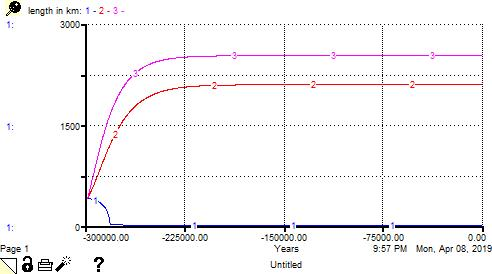
\includegraphics[width=0.8\textwidth]{./p3.jpg}
\end{figure}
\begin{itemize}
\item Warming the climate changes the ``ice sheet-no ice sheet'' threshold.
\item Large ice sheet not possible in warmer climate.
\end{itemize}
}

\frame{
\frametitle{4. Changing the ice strength}
\begin{figure}
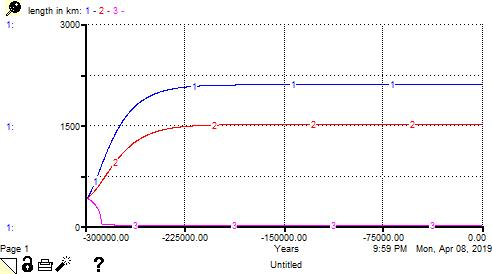
\includegraphics[width=0.8\textwidth]{./p4.jpg}
\end{figure}
\begin{itemize}
\item Reduced ice strength leads to thinner ice and more rapid melting $\rightarrow$ ice sheet disappears
\end{itemize}
}

\frame{
\frametitle{5. Changing ratio of acculumation and ablation rates}
\begin{figure}
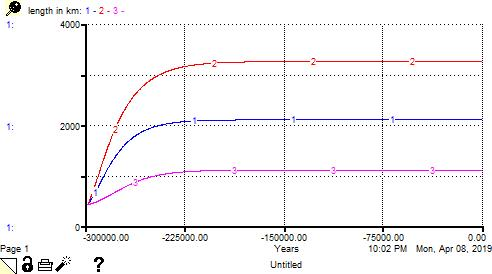
\includegraphics[width=0.8\textwidth]{./p5.jpg}
\end{figure}
\begin{itemize}
\item Ice sheet size increases if the accumulation-to-ablation ratio is increased.
\end{itemize}
}

\frame{
\frametitle{6. Orbital forcing}
\begin{figure}
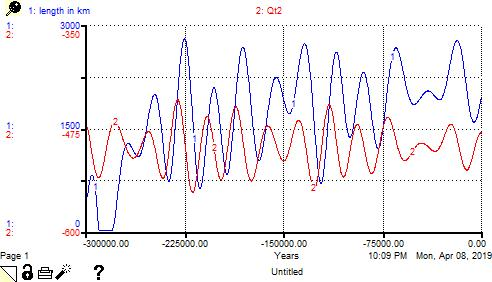
\includegraphics[width=0.8\textwidth]{./p6a.jpg}
\end{figure}
\begin{itemize}
\item Note that I plotted $-Q_t$ to make it more clear that cold periods coincide with large ice sheets.
\item Lag time of a few thousand years.
\item Looks like we should be entering a cool period.
\end{itemize}
}

\frame{
\frametitle{6. Orbital forcing}
\begin{figure}
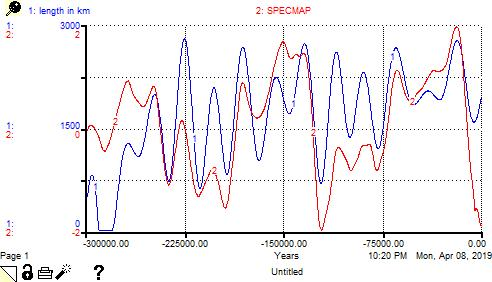
\includegraphics[width=0.8\textwidth]{./p6b.jpg}
\end{figure}
\begin{itemize}
\item Pretty good agreement with SPECMAP (marine isotope record)
\end{itemize}
}

\frame{
\frametitle{7. Feedback loops}
\begin{itemize}
\item \textit{Elevation-climate feedback}: positive feedback loop, in which thickening pushes the ice sheet into a colder climate, which enables more thickening, and vice-versa.
\item \textit{Length-climate feedback}: negative feedback loop, in which increases in length increase the size of the ablation area, leading to increased melting.
\end{itemize}
}

\end{document}

\frame{
\frametitle{Key ideas}
\begin{itemize}
\item System parameters can vary unpredictably as a system evolves toward a steady-state
\item The initial conditions matter $\rightarrow$ systems often have multiple steady states; the initial conditions determine which steady state a system will approach
\item Short pertubations can cause a ``permanent'' transition from one state to another
\item Observed a transition out of the (i) cold state for large perturbations in temperature (ii) warm state for moderate perturbations in temperature
\item Also produced transitions from one state to another by modifying the salinity difference
\end{itemize}
}

\end{document}
